\chapter{Sparky extension for reproducible spectral analysis}
\label{sec_sparky_extension}

\begin{center}
  \textit{The best way to predict the future is to invent it.}

 - Alan Kay
\end{center}


Sparky \cite{sparky} is a popular program for interactive peak picking,
GSS construction, and chemical shift assignment.  Sparky is implemented 
with a C++ core, and Python extensions.  It is designed with
extensibility in mind, with a convenient Python interface through which 
the core data model can be accessed.  The
extensions are also able to augment the user interface with additional
controls, as well as script common operations, and provide extra algorithms
for analysis.  Since Python is a full-featured programming language, 
it is also possible to interact with the filesystem, loading and dumping
data if necessary, as well as calling additional third-party tools.

The extension is intended to help the spectroscopist to capture the 
missing data of analysis: intermediate primary data, extraneous
data, deductive meta data, and notes.  The general approach is to augment
Sparky's data model and user interface with new functionality.



\section{Getting started with Sparky}

\subsection*{Getting Sparky}
A Sparky version including the reproducibility extension can be found at
\url{https://github.com/connjur/SparkyExtensions/releases}.  Simply 
choose the latest version of the correct platform, download it, untar and 
unzip it, and run the sparky executable (in Contents/Resources/bin in the
Mac version, and bin/ in the Linux version).

\subsection*{Dependencies}
The reproducibility extension requires a working git installation in order
to capture snapshots.  git is a freely available tool for version control,
and may be found at \url{http://git-scm.com/downloads}.
git works with local files -- no setup of remote hosts is required.
A git client (a list of which may be found at \url{http://git-scm.com/downloads/guis})
is a useful tool to help view and manage a git repository.  A simple,
cross-platform git client that I have used successfully is "giteye",
which may be found at \url{http://www.collab.net/giteyeapp}.

\subsection*{Sparky manual}
Sparky manuals, which cover the complete use of the program and its many
features in depth, may be found at 
\url{http://www.cgl.ucsf.edu/home/sparky/manual/} and 
\url{http://pine.nmrfam.wisc.edu/PINE-SPARKY/}.

\subsection*{Sparky keyboard shortcuts}
While all Sparky functionality can be accessed through its point-and-click
menu interface, it is far faster to use the keyboard shortcuts, especially
for common tasks.  The most useful of these shortcuts are covered in Table
\ref{sparky_shortcuts}.

\subsection*{Sparky extensions}
Extensions are accessible through the "extensions" pull-down menu,
as shown in Figure \ref{sparky_extensions}.
Additionally, the reproducibility extension is accessible through
the "re" shortcut (see Figure \ref{sparky_reproducibility}),
and the "rg" shortcut brings up the group editor.



\section{Concepts}
Automated algorithms do not usually produce perfect results in NMR analysis.
Automated peak picking,
GSS construction, and GSS-residue assignment need manual validation and
correction.  These manual modifications are inherently difficult, tedious,
and error-prone because they are the most complicated to correctly analyze.
However, correctly analyzing them has an important impact on the quality
of the final result.
The main goal of this extension is to facilitate reproducibility
by capturing the entire analysis process, including manual modifications.

The process of manual analysis is composed of a series of discrete steps.
At each step, a deductive rule is applied to the data set, producing a
modified new data set.  Thus, for each rule, knowing the context is important:
it allows one to determine how appropriate the application of a specific rule
is, as well as what the results should be, and to determine whether the 
results are consistent with expectations.

\subsection*{GSS and resonance}
Sparky's data model is shown in Figure \ref{sparky_model}.  It includes 
entities for spectra, peaks, resonances, GSS, atoms, and molecules, among
others.  Sparky does not natively distinguish between a GSS (generic spin 
system) and a residue, nor between a resonance and an atom.

Both GSSs and resonances have been implemented in the extension, based 
on the CCPN model \cite{ccpn}.

\subsection*{Extraneous data}
In standard analysis, false positive peaks (picked as true peaks initially,
but later determined to be noise or artifactual) and false positive spin 
systems (not assigned to any residue) are typically deleted and/or ignored.
In this extension, \textbf{data is never deleted}.  Such results are kept,
since they have valuable information content, even if they are not used for
the immediate purpose of the analysis process (be it structure or dynamics
determination).  These results are kept by, instead of deleting them, 
explicitly marking them as not of interest, and placed in a different
category.

\subsection*{Snapshots}
Snapshots of intermediate states during analysis are used to enable rehashing
of the deductive process.  In general, by capturing a snapshot of the data set
each time a deductive rule is applied, the context of each manual modification
is captured.

An additional benefit of capturing snapshots is that they allow one to go 
backward in time.  This is useful for understanding what happened and
why, but is also useful for fixing mistakes and accidents -- this is
important because Sparky can not undo changes.
If a datum is accidentally changed, it may not even be noticed, and it is 
impossible to easily restore.  Capturing snapshots trivially solves both
of these problems.

\subsection*{Deductive reasoning}
Capturing the deductive rules applied during the process of manual assignment
provides semantic information about what is being done and why.  This makes it
far more meaningful to examine the sequence of snapshots of an analysis
process and determine the context.



\section{Project setup}
From the terminal, create an empty directory and "cd" into it.
Intialize it as an empty git repository and create the Sparky directory
structure with the following terminal commands:
\begin{verbatim}
$ git init
$ mkdir Projects/
$ mkdir Save/
$ mkdir Data/
\end{verbatim} 
Make sure to save all spectra files in the "Data/" directory.
When in Sparky, save the project in the "Projects/" directory.
The Sparky .save files will automatically be written into the "Save/"
directory.

Now start Sparky and take care of tedious initial project setup.  This includes:
\begin{itemize}
  \item opening each of the spectra that will be used (using the "fo" shortcut)
  \item setting the contour levels ("ct").  Some nice default setting are
    "15 levels" for both positive and negative contours, and "red-yellow" color
    for positives, along with "blue-green" for negatives
  \item setting the ornament and label sizes ("ot" and "oz")
  \item setting the visible depth
  \item getting the axes in the correct order ("xx" and "xr")
  \item setting the aspect of each spectrum appropriately ("yt")
  \item syncing axes of identical nuclei.  For example, the 1H axes of
    an NHSQC, HNCACB, HN(CO)CACB, HNCO, and C(CO)NH-Tocsy should be synced; 
    similarly, all their 15N axes should be synced as well.  However, the
    13C axis of an HNCACB and an HNCO should not be synced, although the
    13C axis of an HNCACB and a C(CO)NH-Tocsy should by synced
\end{itemize}
Now it is time to take a snapshot of this configuration.

\section{Capturing a snapshot}
Whenever a snapshot is desired, this procedure must be followed:
\begin{itemize}
  \item save the project ("js")
  \item type in the appropriate deductive reason in the "deductive reason used"
    text box, or whatever annotation accurately describes the purpose of the 
    snapshot
  \item click the "make snapshot" button
\end{itemize}
This will use git to create a new snapshot.  At any time, the contents of
the git repo can be examined using the terminal and the file browser.  Git
supports many features for examining and manipulating history.  These may
all be accessed from the terminal.

% TODO does this paragraph make any sense?
Snapshots provide a record of the process of analysis.  By capturing snapshots
at appropriate intervals, effective perusal of the process at a later date is
enabled.  A more immediate benefit is the ability undo mistakes, which is 
important because most mistakes can not be undone using Sparky.
In general, it is necessary to capture a snapshot immediately after
running an automated tool and before making any manual modifications.  During
manual analysis, capturing a snapshot after each focused sub-goal is necessary.



\section{Reproducible backbone assignment tutorial}
There is a nice tutorial and dataset in Sparky format at 
\url{http://www.nmr.chem.uu.nl/~abonvin/tutorials/Assignment-Data/assignment.html}.
It includes the NHSQC, HNCACB, and HN(CO)CACB of a small protein -- enough
to carry out sequential backbone assignments.
This section will show how to reproducibly make these chemical shift
assignments.

\subsection*{NHSQC peak picking}
Use standard Sparky facilities to peak pick your NHSQC spectrum.
First, make sure to set the contour levels high enough that few noise and 
artifact peaks will be picked, but low enough that most true signal peaks
will be picked.

\subsection*{NHSQC cleanup: signal/noise/artifact identification}
Some of the peaks Sparky found will turn out to be noise or artifact peaks.
\textbf{Do not delete peaks, ever, for any reason!}  Instead,
when peaks are identified as such, select them and press the "Set selected 
peaks to noise" or "Set selected peaks to artifact" button, as necessary.
Peaks must not be assigned when setting them to noise or artifact.

Sparky will not find all true peaks.  Whenever a true signal is found 
unpicked, simply pick the peak manually by switching the cursor mode to 
"find/add peak" and using "pc" to center the peaks after they have been
picked.

Overlapped peaks are also a problem.  They may cause too few peaks to be 
picked, or peaks to be picked in a slightly wrong position.  If these errors
can be rectified manually, simply add peaks and move others as necessary.

Either a restricted peak pick (using NHSQC peaks) or a standard peak pick
of the full dimensions should be used to peak pick all other N-H-rooted
spectra (such as the HNCO, HNCACB, CCONH-Tocsy, etc.).

\subsection*{GSS initialization}
It is convenient to create one GSS for each NHSQC peak that is or may be
a signal peak.  Select the NHSQC peaks which will be used as GSS roots.  
All signal peaks can be selected using the "select signal peaks" drop-down.
Then press the "create new group for peak" button.

When an NHSQC peak is used to initialize a GSS, the GSS will start off
with two resonances: one for the H, and one for the N.

\subsection*{GSS construction}
Open the peak-GSS assignment dialog by pressing the "Open peak-GSS dialog"
at the bottom of the reproducibility window.

Now set up the parameters by choosing the spectra from which peaks will
be used as GSS roots (typically the NHSQC) and that which has the peaks to
be assigned.  Make sure the desired dimensions are matched and set the 
tolerances appropriately; I typically use 0.2 PPM for a 15N axis and 0.02 PPM
for a 1H axis but this can vary based on the alignment between spectra.
Finally, select all the peaks in the "from" spectrum that should be used;
you can select all signal peaks using the "select signal peaks" drop-down.

The way that GSS construction works is that for each peak in the "from"
spectrum, all peaks in the "to" spectrum within the tolerances will be
assigned to the same GSS as the "from" peak.  Peaks in the "to" spectrum that
match 0 "from" peaks will not be assigned to any GSS; those that match more
than 1 peak will also not be assigned, but a warning will be generated in
the shell, allowing manual resolution.

Matching requires that some subset of the spectral dimensions match.  Using
an NHSQC and an HNCACB, the H and the N dimensions match.  The resonance
assignments of the peak cross sections will be carried over for matching dimensions,
and new resonances will be created for the C dimension.

\subsection*{Peak cross section to resonance assignment}
A resonance is assigned to each cross section of each group which is in a GSS.
If a peak cross section has a unique chemical shift value within a GSS, it will
be the only one assigned to that resonance; if multiple cross sections share 
the same or similar chemical shift value, they will be assigned to the same
resonance.  This reflects the fundamental NMR property that an atom resonates
at the same frequency across spectra. 

Peak cross section to resonance assignment can fail in two cases, and these
can be resolved by manually modifying the assignments to resonances.

First, when the chemical shifts between the peak cross sections do not match
within the tolerances, multiple resonances are created.  These can be merged
using the built-in Sparky assignment tools by changing the assignment of one
peak cross section to match the other.
Second, in the case of overlap, a single resonance is created when there
should actually be multiple resonances.  This can also be resolved using 
the built-in Sparky assignment tools, by simply changing the assignment of
one peak dimention to a fresh resonance id.

\subsection*{Changing peak-GSS assignments}
There are two major cases for moving a peak from one GSS to another.
First, for GSS types such as Q and N sidechains, there are usually multiple
peaks in the NHSQC (because of the two protons).  Simply select the appropriate
peaks, choose a GSS id (typically the lowest of the GSS ids of the selected
peaks, just for convenience and consistency) and press the "set groups of
selected peaks" button.
Second, peaks may be assigned to the wrong GSS.  Select the incorrect peaks,
type in the desired GSS id, and press the "set groups of selected peaks" button.

\subsection*{Resonance typing}
The types of resonances are assigned using BMRB statistics, GSS typing, 
peak characteristics,
and the pulse sequences of the spectra in which they appear.  For some spectra,
such as the NHSQC, there are relatively few choices: for backbone GSSs,
the resonance types are always amide-H and amide-N.  However, other spectra
have more choices: for the HNCACB, resonances in backbone GSSs in the C
dimension can be CA, CA(i-1), CB, or CB(i-1).

There are two ways to assign resonance types.  First, each resonance assigned
to a peak's cross sections a peak may be assigned at once.  The possibilities
for these resonance typings are called "peaktypes" and depend on the pulse 
sequence of the spectrum in which the peak is found.
This can be done using "assign peaktype" drop-down menu.  Select the correct
spectrum, which will bring up a list of possible peaktypes which may be found
in that spectrum.  Make sure to set the dimension order properly.

The second way is to assign resonance types individually.  This can be done 
using the keyboard shortcut "rg" to bring up a group/resonance editor
(see Figure \ref{sparky_reproducibility}).  Clicking on a group will allow
for editing of group assignments, while clicking on a resonance allows for
resonance typing.

Ambiguous resonance typings are also supported.  Common examples include
CA/CA(i-1), HA2/HA3 (Glycine), HB2/HB3 (many amino acids), and QB (Alanine).

\subsection*{GSS typing, sequential, and sequence-specific assignment}
GSSs are assigned types based on BMRB statistics, the presence or absence of
characteristics resonance types, and possibly also based on the assignments 
of linked GSSs.
GSS types for H-N-rooted GSSs include backbone types for each of the 20 
standard amino acids, as well as sidechain types for Q, N, R, W, and K.

Sequential GSS assignments are identified based on overlapping compatible
resonances between GSSs: for example, a GSS with a CA at 58.32 PPM and a CB
at 30.27 PPM, and a second GSS with a CA(i-1) at 58.21 and a CB(i-1) at 30.41:
these GSSs have overlapping compatible resonances and can be sequentially
assigned.
It is not necessary that resonance types are unambiguously assigned before
doing sequential GSS assignments: if it is unclear whether a resonance is a
CA or CA(i-1), this may be assigned simultaneously as the sequential assignment
is made, if it is consistent with the overlap from the other GSS.

Additionally, sequential GSS assignment can lead to the picking of additional
peaks, or the resolution of GSS overlap, if such picking and/or resolution
leads to consistent and compatible overlap with another GSS.
GSSs are assigned to residues on the basis of GSS typing, sequential GSS
assignments, and the primary sequence.

GSS assignment is accomplished using the "group editor" dialog by clicking on
the appropriate group.  This will bring up a dialog which allows typing,
sequential assignment, and sequence-specific assignment.



\section{Pitfalls}
Sparky's data model was extended to support reproducible analysis.
However, it is possible to circumvent the extension's model and assign peaks
and resonances differently. If care is not taken when doing so, the data
may be incompatible with the extension.

\section{Creating an NMR-STAR file}
While the data is stored as standard Sparky-formatted files in a git repository
during analysis for convenience, after analysis is complete, the project
may be converted to a single NMR-STAR file, containing the complete history
of the project.  This conversion may be accomplished using a tool which
automatically extracts each snapshot version from the git repository, 
parses the snapshot into a data structure,
calculates semantic diffs between successive snapshots, 
and finally generates an NMR-STAR file containing the data.

 

% tables
\clearpage
\section{Tables}

\begin{table}[h]
  \begin{tabular}{ | c | c | }
    \hline
    shortcut    &   effect                  \\  \hline
    ct      &  open contour dialog          \\  \hline
    yt      &  open spectrum dialog         \\  \hline
    pc      &  center peak                  \\  \hline
    aD      &  delete peak assignment       \\  \hline
    re      &  open reproducibility dialog  \\  \hline
    rg      &  open group editor dialog     \\  \hline
    ot      &  ornament settings            \\  \hline
    xr      &  roll axes                    \\  \hline
    xx      &  transpose axes               \\  \hline
    jo      &  open project                 \\  \hline
    jc      &  close project                \\  \hline
    js      &  save project                 \\  \hline
    fo      &  open spectrum                \\  \hline
    py      &  open Python interpreter      \\  \hline
  \end{tabular}
  \caption{Important Sparky keyboard shortcuts.}
  \label{sparky_shortcuts}
\end{table}



% figures
\clearpage
\section{Figures}

\begin{figure}[h]
  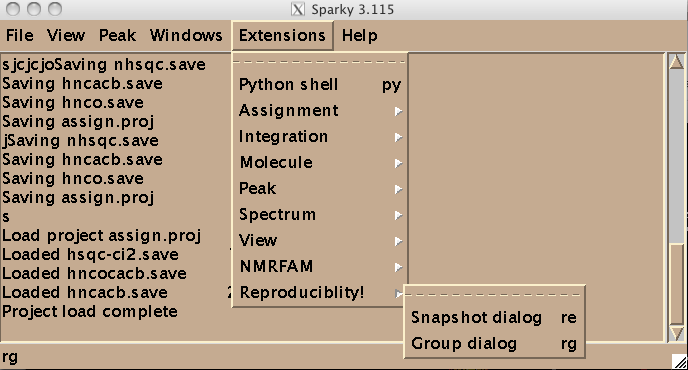
\includegraphics[scale=0.6]{figures/sparky_extensions}
  \caption{The Sparky interface, showing how to activate the reproducibility
           extension.}
  \label{sparky_extensions}
\end{figure}

\begin{figure}
  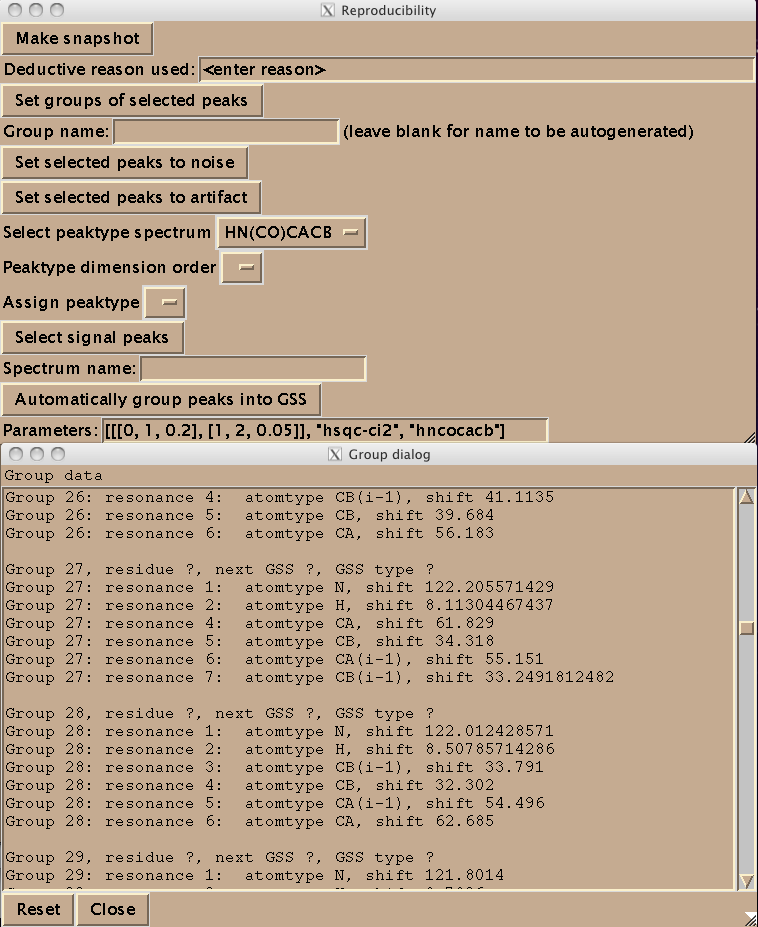
\includegraphics[scale=0.5]{figures/sparky_reproducibility}
  \caption[Two widgets provided by the reproducibility extension.]
          {Two widgets provided by the reproducibility extension.
           The first provides core functionality for making snapshots,
           annotating snapshots, and creating and building GSSs, as
           well as assigning peaktypes.  The second provides functionality
           for displaying, assigning and merging GSSs and resonances.}
  \label{sparky_reproducibility}
\end{figure}

\begin{figure}
  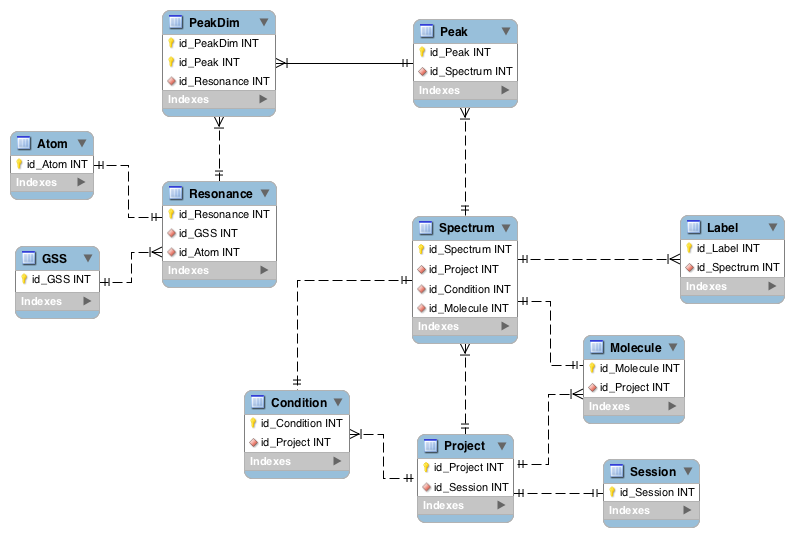
\includegraphics[scale=0.5]{figures/sparky_model}
  \caption[The Sparky data model]
          {The Sparky data model showing the key relationships.
           These data are available from within Sparky extensions.
           The model was created in MySQLWorkbench.}
  \label{sparky_model}
\end{figure}

